
\section{Reflective Practicioner}
\label{sec:RP}
\subsection{Introductie}
Voor het onderzoeksgedeelte heb ik mij gericht op wat studenten en docenten als meest waardevol beschouwen in de les. Waar hebben ze het meeste van geleerd, ten opzichte van waarvan de docenten denken wat het meest waardevol is om te doen. De onderzoeksvraag is:
\begin{quote}
  "Hoe verschillend zijn de zienswijze van student en docent ten opzichte van onderwijs en de rol van de docent daarin?"
\end{quote}
De onderzoeksvraag is ontstaan door een interesse die gewekt is na het lezen van een aantal meta-analyses in het onderwijs-onderzoeksveld \cite{hattie2008visible, schneiderVariables}. Beiden analyses die noemen eigenlijk dat de meeste onderwijsmethoden een positief effect hebben op leren, zolang er maar lesgegeven wordt. Maar er zijn sommige die een veel grotere impact hebben dan anderen, zoals: open vragen t.o.v. gesloten vragen stellen, sleutelwoorden op slides zetten t.o.v. volzinnen \cite{schneiderVariables}. Omdat student en docent het onderwijs wat ze volgen of geven heel anders ervaren, is het interessant om te kijken of hoe groot de verschillen zijn in wat beiden partijen waarnemen als methoden die het leereffect verhogen. Niet puur uit een wetenschappelijke interesse, maar ook om dat weer te gebruiken in de praktijk.

\begin{figure}[h]
	\centering
	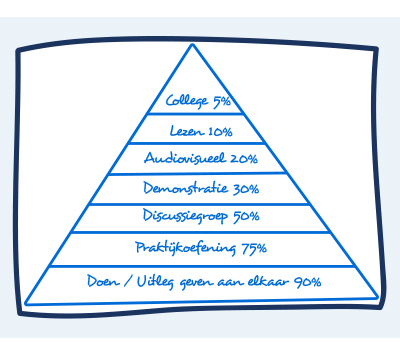
\includegraphics[width=4in]{piramidevanbales}
	\caption{Piramide van Bales.}
\end{figure}

Daarbij wil ik verschillende thema's afgaan: colleges, hoe ``leuk'' een les is, het tempo, persoonlijke begeleiding, plenaire of klassikale momenten en taken opgegeven door een docent. Vooral de colleges en klassikale momenten vond ik interessant om onder de loep te nemen omdat volgens de leercone van Dale die heeft geleid tot de leerpiramide van Bales, colleges tot zeer weinig retentie zou leiden \cite{leerpiramidebales}. De illusie dat er maar 5\% wordt opgevangen bij een college volgens de leerpiramide van Dale is in duigen gevallen door verschillende onderzoeken samengevat door Lalley \& Miller, die aantonen dat het wel degelijk aangetoond tot retentie kan leiden \cite{lalley2007learning}. Zoals alles in context en doel belangrijk.

\subsection{Methodiek}
Aan de hand van een vragenlijst die beschreven staan in \hyperref[sec:vragenlijstRP]{Bijlage E - Vragenlijsten} heb ik geprobeerd te kijken wat de verschillen zijn tussen studenten en docenten door dezelfde onderwerpen vragen in een vraag geformuleerd voor de student en één geformuleerd voor de docent. Het is niet een wetenschappelijk opgestelde vragenlijst, noch zal de analyse een wetenschappelijke aard hebben.

De vragen zijn op een schaal van nooit-altijd beantwoord. Bij sommige van de vragen heb ik alle antwoorden die positief/negatief zijn bij elkaar gegooid het onderscheid daartussen iets scherper te krijgen.

Voor de studie heb ik het woord ``leuk'' gebruikt in de vragenlijst, daar vallen mensen wellicht over, maar het belangrijkste is naar mijn mening dat de interesse gewekt is en er een urgentie-besef is voor de student die intrinsieke motivatie oplevert om zelf te leren zoals Dochy beschrijft in de HIL(L)-methode \cite{dochy2015high}.

\subsection{Bevindingen}
Ten eerste is mij duidelijk dat de vragen die ik heb gesteld niet altijd duidelijk waren, en in sommige opzichten onvolledig. Dus ik zal het even moeten doen met de vragen die gesteld zijn. 

\subsubsection{Colleges}
Eigenlijk zijn zowel studenten (92.6\%) en docenten (100\%) het er mee eens dat de colleges meer dan soms nuttig zijn. Opvallend is dan wel dat bijna de helft van de studenten (43.1\%) vindt dat zij overwegend niet veel hoeven in te halen als ze een college gemist hebben, terwijl de docenten (90\%) dat overwegend wel vinden.

\subsubsection{``Leuk'' (ofwel intrinsieke motivatie)}
Alle docenten proberen over het algemeen het vak leuk te maken (100\%), de meeste studenten (87\%) vinden dat een docent daar ook in bepalend kan zijn voor een vak. En daarin hebben juist docenten (100\%) vaker het idee dat dat effect heeft dan studenten (92\%).

\subsubsection{Tempo}
Het meest verdeeld lijken de studenten en docenten over het tempo van de les. Als een docent te snel gaat dan haakt 51.3\% soms niet/wel, 18.8\% vaak en 8.8\% altijd af. Terwijl als een docent te langzaam gaat haakt 50\% soms niet/wel, 18.8\% vaak en 11.3\% altijd af.

Het lastige hierbij is dat van de docenten 61\% aangeeft niet altijd door te hebben dat ze te snel gaan en daarmee de studenten af haken. En ongeveer evenveel (60\%) docenten aangeven niet altijd gas terug te nemen als ze te snel gaan.

\subsubsection{Persoonlijke begeleiding}
De meeste studenten (93.6\%) zoeken zelf iets uit als iets niet snappen, waarbij ook de meesten meestal om hulp vragen als ze er niet uitkomen (93.9\%), dit komt ook wel overeen met hoe de docenten er naar kijken. Het overgrote gedeelte laat de studenten zelf ploeteren (88.9\%) terwijl de meeste ook denken dat een student om hulp vraagt als een student er niet uitkomt (93.4\%).

Van de studenten geeft 10.1\% aan dat het meestal niet helpt als een docent bij ze komt zitten om iets uit te leggen, terwijl geen een van de docenten dit lijkt in te zien (0\%!).

\subsubsection{Klassikaal}
De klassikale momenten van uitleg zijn in onze ``flipped classroom'' inmiddels niet zo heilig meer, maar toch denkt 94.4\% van de docenten dat het meestal duidelijk is na een klassikale uitleg. Terwijl 26.3\% van de studenten vinden dat ze meestal niet veel leren als een docent iets klassikaal uitlegt. Met nog eens 40\% van de studenten die dat ze meestal iets leren, maar niet altijd.
Wat wel opvallend is is dat er ook maar minder dan de helft studenten meeschrijven met een docent, slechts 46.2\% van de studenten geeft aan soms of meestal mee te schrijven.

\subsubsection{Docent geeft opdracht om aan te werken}
Alle docenten vinden dat wanneer ze studenten aan het werk zetten de studenten veel leren, de meeste studenten 89.7\% vinden ook dat dat meestal het geval is.

\subsection{Conclusie \& Discussie}

Onderzoek vertelt ons dat een docent hoeft maar op een manier instructies hoeft te geven en het heeft al een positief leereffect, toch zijn er dingend die meer effect lijken te hebben \cite{hattie2008visible}. Zo zijn momenten van 1-op-1-begeleiding en studenten zelf laten beoordelen en uitleggen een aantal uitspringers volgens onderzoek \cite{schneiderVariables, hattie2008visible}.

Maar wat zijn nou dingen die opvallen in deze resultaten omdat ze zo verschillend worden bekeken door student en docent?

In de resultaten komen een aantal grote verschillen naar voren bij de onderwerpen: colleges, tempo en de klassikale momenten. Misschien ook wel de meest ingewikkelde moment om te faciliteren, sommige mensen lopen voor anderen weer achter.

Een meer merkwaardig resultaat is misschien wel dat iedereen het erover eens is dat de colleges wel zin hebben, maar dat student en docent er heel anders naar kijken hoeveel het werk er in te vallen valt na een gemiste les. Docenten zeggen allemaal dat er hier wel werk bij komt kijken, terwijl 43.1\% van de studenten, dat gevoel niet lijkt te delen. Wellicht houden het tempo en de `nuttigheid' van de colleges ook wel met elkaar verband. In ieder geval wil ik speculeren dat ze verband houden met feit dat een kwart van de studenten aangeven niet iets te leren van een klassikale uitleg. Het zal hier voor de studenten niet helpen dat ze overwegend niet meeschrijven. Dit zal de retentie en het leereffect van de colleges zeker helpen.

De docenten geven aan niet gas terug te nemen, terwijl ze door hebben dat ze te snel geven en de studenten geven aan dat ze dan niet meer betrokken zijn bij de les. Het aantal studenten wat afhaakt als het te langzaam gaat zit ongeveer rond hetzelfde percentage. Hoe kan een docent hier rekening mee houden? Een klassikaal moment is natuurlijk ook lastig, veel niveauverschillen. In die zin kan je nooit iedereen tevreden houden. Maar toch zou men als docent graag hier in iets willen betekenen voor de studenten. Een conclusief en finaal antwoord kan ik hier niet voor bieden. Wel heb ik een manier gevonden waarin ik het idee heb dat ik invloed kan uitoefenen op de participatie in de les.

\subsubsection{Suggesties voor de participatie }
Aan het begin van een lesperiode (na ongeveer 2 á 3 weken in een lesperiode van 2 maanden) probeer ik graag te polsen hoe de lesstof en de lessen worden ervaren aan de hand van een korte vragenlijst, ik vraag hierin ook om tips en wat ze graag anders zouden willen zien. De resultaten van deze korte vragenlijst bespreek ik tijdens de les met de studenten. Ik heb het idee dat ik hiermee een gevoel van inspraak en zeggenschap kan creëeren terwijl ik ook mijzelf open stel voor verbetering. Wanneer hier ruimte voor is krijg ik het idee dat er ook wederzijds ruimte is voor feedback op de les, maar ook op het leren. Dan probeer ik aan te geven wat strategieën zijn die werken, en op wat voor beoordeling ze af stevenen als het zo verder gaat.

Als ik ook kijk naar de beoordelingen van de studenten, de participatiegraad, de aanwezigheid en de eindcijfers, dan denk ik dat ik boven het gemiddelde heb gescoord de afgelopen periode waar ik dit gesprek ben aangegaan. Nou is het altijd lastig aan te geven waardoor dit nou precies komt, maar ik denk zeker als docent ook daarin mijn stempel te hebben kunnen drukken. 